\documentclass[12 pt, a4paper]{report}
\usepackage[utf8]{inputenc}
\usepackage[T1]{fontenc}
\usepackage{hyperref}
\usepackage{todonotes}
\usepackage{gensymb} % superscript
\usepackage{textcomp} % superscript
\usepackage{amsmath} % symboles des degrés

% --------------------  NOMBRES ET UNITÉS ---------------------------
\usepackage{siunitx}
\iffalse % explication des fonctions courantes
The package provides the user macros:
• \ang[hoptionsi]{hanglei}
• \num[hoptionsi]{hnumberi}
• \si[hoptionsi]{huniti}
• \SI[hoptionsi]{hnumberi}[hpre-uniti]{huniti}
• \numlist[hoptionsi]{hnumbersi}
• \numrange[hoptionsi]{hnumbersi}{hnumber2i}
• \SIlist[hoptionsi]{hnumbersi}{huniti}
• \SIrange[hoptionsi]{hnumber1i}{hnumber2i}{huniti}
• \sisetup{hoptionsi}
• \tablenum[hoptionsi]{hnumberi}
plus the S and s column types for decimal alignments and units in tabular environments.
12 345.678 90        \num{12345,67890}
1 ± 2i               \num{1+-2i}
0.3 × 1045           \num{.3e45}
1.654 × 2.34 × 3.430 \num{1.654 x 2.34 x 3.430}

\si{kg.m.s^{-1}}
kg m s−1
Simple lists and ranges of numbers can be handled.
\numlist{10;20;30} \\
\SIlist{0.13;0.67;0.80}{\milli\metre} \\
\numrange{10}{20} \\
\SIrange{0.13}{0.67}{\milli\metre}
10, 20 and 30
0.13 mm, 0.67 mm and 0.80 mm
10 to 20
0.13 mm to 0.67 mm

\ohm\metre
\celsius

\fi
% --------------------------------------------------------------

\usepackage{hyperref}

\usepackage{natbib}       % Pour la bibliographie
\usepackage[french]{babel}
\usepackage{graphicx}     % Pour les figures
\usepackage[toc]{appendix}% Pour les annexes
\usepackage{titlesec}     % Pour modifier les titres
\usepackage{fancyhdr}     % Pour les haut et bas de pages (numéros)
\usepackage{lipsum}       % Rajoute du texte temporaire
\usepackage{parskip}      % Modifie l'apparence des paragraphes
\usepackage{setspace}     % Pour interligne et demi
\usepackage{listings}     % Pour afficher du code sans formattage

\selectlanguage{french}

% ------------------------- COMMANDES -------------------------------

\newcommand\var[2]{\newcommand{#1}{\ensuremath{#2}}}
% C'est pratique de définir des variables au début pour éviter de
% réécrire des formules et cela facilite modifier l'affichage.

\makeatletter
\newcommand{\makecustomtitle}{
  \newpage
  \null
  \begin{center}
  \let \footnote \thanks
    {\LARGE \textbf{\@title} \par}
    \vskip 1em
    {\large \@date \par}
    \rule{1.5in}{0.4pt}
  \end{center}
  \par
}
\makeatother


\bibliographystyle{abbrvnat}
\setcitestyle{authoryear,open={(},close={)}}

% Renomme les noms par défauts pour qu'ils soient en français
\renewcommand{\contentsname}{Table des matières}
\renewcommand{\listfigurename}{Liste des figures}
\renewcommand{\listtablename}{Liste des tableaux}
\renewcommand{\appendixname}{Annexe}
\renewcommand{\appendixtocname}{Annexes}

%% ------------------------ NUMÉROS DE PAGE --------------------------
\fancyhf{} % clear all header and footers
\renewcommand{\headrulewidth}{0pt} % remove the header rule
\rhead{\thepage}
\pagestyle{fancy}
\setlength{\headheight}{15pt}

\makeatletter % Un hack pour les numéros de page
\renewcommand\chapter{\if@openright\cleardoublepage\else\clearpage\fi
                    \thispagestyle{fancy}%
                    \global\@topnum\z@
                    \@afterindentfalse
                    \secdef\@chapter\@schapter}
\makeatother

%% --------------------------- TITRES ---------------------------------
\renewcommand{\chaptername}{}
\titleclass{\chapter}{straight}
\titleformat{\chapter}
[hang]
{\raggedright\normalfont\Large\bfseries}
{\filright\MakeUppercase{\chaptertitlename} \Large\thechapter\ - }
{0pt}
{\Large\MakeUppercase}

%% ------------------------- VARIABLES ---------------------------------
\newcommand\var[2]{\newcommand{#1}{\ensuremath{#2}}}
% C'est pratique de définir des variables au début pour éviter de
% réécrire des formules et cela facilite modifier l'affichage.
\var\Fx{F_x}
\var\Fy{F_y}
\var\vF{\rm\bf F}
\var\Fmin{F_{\rm min}}
\var\Fmax{F_{\rm max}}

%% ------------------------ document commence --------------------------
\begin{document}

\begin{titlepage}
    \begin{center}
        \large
        DÉPARTEMENT DE GÉNIE MÉCANIQUE\\
        Faculté de génie\\
        Université de Sherbrooke\\
        
        \vspace{3cm}
 
        \Huge
        \textbf{Gabarit \LaTeX}
        
        \large
 
        \vspace{3cm}
 
        par\\
        Équipe 1\\
        TOMMY ALPHA\\
        TOMMY BETA\\
        TOMMY CHARLIE\\
        TOMMY DELTA\\
        TOMMY EPSILON\\
        TOMMY FARADAY\\
 
        \vfill
 
        Travail présenté à\\
        ORGANISATION
 
        \vspace{1.5cm}
 
        %\includegraphics[width=0.4\textwidth]{university}
 
        \Large
        Sherbrooke\\
        1 JANVIER 2019
 
    \end{center}
\end{titlepage}

\onehalfspacing
\chapter*{Sommaire}
\lipsum[1-2] % texte temporaire à remplacer

\pagebreak

\singlespacing
\tableofcontents
\pagebreak

\onehalfspacing
\addcontentsline{toc}{chapter}{\listfigurename}
\listoffigures
\addcontentsline{toc}{chapter}{\listtablename}
\renewcommand{\tablename}{Tableau} % Table ou Tableau
\renewcommand{\thetable}{\arabic{table}}
\listoftables
% --------------------- LISTE DE VARIABLES ----------------------
\addcontentsline{toc}{chapter}{Liste de variables}
\chapter*{Liste de variables}

\begin{tabular}{ l l }
% nom & description \\
\Fx & La force en $x$\\
\Fy & La force en $y$\\
\Fmin & La force minimale\\
{$\theta$} & L'angle theta\\
\vF & Le vecteur de la force\\
\end{tabular}

\addcontentsline{toc}{chapter}{Liste d'abréviations}
\chapter*{Liste d'abréviations}
\pagebreak

\chapter{Introduction}
\lipsum[4-6] % texte temporaire à remplacer

\pagebreak

\chapter{Problématique}
\lipsum[1-1]
\chapter{Objectifs}
\lipsum[2-2]

\pagebreak

\chapter{État des connaissances}
\lipsum[1-1]
\section{Méthodologie}
\lipsum[2-2]
\subsection{Sous-section}
\lipsum[3-5]
\section{Résultats}
\lipsum[6-7]

\chapter{Fonctions \LaTeX}

On déclare les variables au début. Après on peut les utiliser comme \Fx\ ou \Fy, ou encore \Fmax, ou encore le vecteur \vF. Ça marche après dans une équation aussi.

\begin{equation}
    \Fx = 0
\end{equation}

\begin{figure}[ht!]
\centering
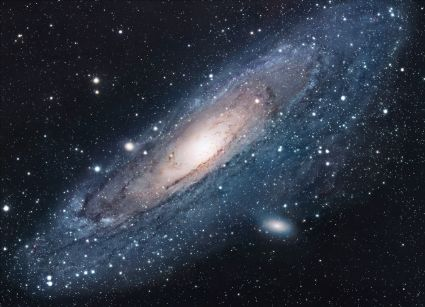
\includegraphics[scale=1.7]{universe}
\caption{The Universe}
\label{fig:universe}
\end{figure}

«I always thought something was fundamentally wrong with the universe» \citep{adams1995hitchhiker}

\lipsum[1-1]

\pagebreak

\chapter{Conclusion}
\lipsum[1-2]

\begin{appendices}
\chapter{Aide-mémoire des fonctions \LaTeX}
Voici des tables contenant les fontions \LaTeX les plus utilisés. La table \ref{table:nomDeRef} présente les fonctions de traitement de textes. 

\begin{table}[h!]
\centering
\caption{Table to test captions and labels}
\begin{tabular}{|c | c|} 
 \hline
 Col1 & Description \\ [0.5ex] 
 \hline
 1 & 6 \\ 
 2 & 7 \\
 3 & 545 \\
 4 & 545 \\
 5 & 88 \\ [1ex] 
 \hline
\end{tabular}
\label{table:nomDeRef}
\end{table}

\chapter{Fragments de code \LaTeX}
 
This text is again outside the environment

\end{appendices}

\pagebreak

\bibliographystyle{plain}
\bibliography{references}
\newpage
\end{document}
